
    The research contributions of this thesis are based on a novel constraint
    programming approach on compiler intermediate representation.
    This chapter introduces the theoretical underpinnings of this approach,
    based on a mathematical model of static single assignment form (SSA).
    With the help of this model, concepts that are typically discussed on a
    programming language level are transferred onto the structurally simple,
    but semtantically expressive class of SSA compiler intermediate
    representations.

    Constraint formulas on SSA respresentations initially appear to mimic
    pattern matching approaches on abstract syntax tree (AST) level.
    However, they quickly prove themselves to be vastly more expressive.
    Some consideration is necessary to handle search space explosion, but
    the reward are much more powerful recognition capabilities and the
    expression of higher level algorithmic structures, which are impossible to
    define syntactically on programming language level.
    Later chapters will explore the power of this approach in detail, by
    building a complete constraint programming language on top of the theory in
    this chapter, and by then using it to solve real compiler analysis problems.

    After defining a mathematical foundation of SSA form and introducing
    formalisms for the expression of basic contraint problems on top of it,
    several standard definitions from compiler theory are reformulated in the
    framework.
    This includes common graph properties, including the concept of domination,
    as well as control flow structures such as single entry single exit blocks.
    All of this lays the foundations for the succeeding chapter.

    Finally, for the practical application of constraint programming to compiler
    intermediate representation, efficient solver techniques are required.
    The last section in this chapter discusses strategies for limiting
    compile time explosion and explores analogies of the described model to
    standard Satisfiability Modulo Theory (SMT) problems.
    This gives further insights into performance improvements and puts the
    work into a broader theoretical context.

\section{Introduction}

    Modern compilers for procedural languages such as
    C/C++, Fortran or JavaScript typically use a succession of different
    representations for the program during compilation.
    They can be grouped into categories and reflect the requirements of
    the compilation stages they are used in.
    \linebreak
    {\bf Front end representations} are close to the source program and
    naturally reflect the internals of the compiler front end, especially the
    parser.
    Typically, they are built on an abstract syntax tree representation with
    additional annotations, such as type information.
    In addition to encoding program logic, these representations are rich in
    information about syntactic and  stylistic choices of the programmer.
    They scale in complexity with the source language and further obscure the
    program semantics by not resolving complex language features, such as
    operator overloading.
    \linebreak
    {\bf Back end representations} are based on a model of the target hardware.
    These representations typically approach an assembly style format,
    exposing specific instruction set architectures of the hardware.
    Back end representations are concerned with problems that are removed from
    the algorithmic core of the user program, such as register allocation and
    instruction scheduling.
    \\
    {\bf Static Single Assignment} (SSA) form has emerged as a suitable
    representation in the middle end, which is traditionally responsible for
    applying complex optimising transformations.
    SSA abstracts away the complexities of both the source language and the
    target architecture, instead focusing on a relatively simple semantic
    description of the user program that enables reliable analysis and platform
    independent reasoning.
    It is these properties that also make it the suitable target for expressing
    algorithmic structures.

    Static Single Assignment is not a strictly defined or mathematically
    codified standard, but instead refers to a group of representations that
    share important characteristics,
    the eponymous SSA property being only one among them.
    Instruction sets, syntax and type systems of the different
    SSA intermediate representations vary considerably, depending on the
    requirements of the source languages (static or dynamic)
    and the operating constraints (just-in-time or ahead-of-time).
    Some prominent examples of compilers that utilize SSA for their
    optimisation passes include {\bf clang} (LLVM IR), {\bf gcc} (GIMPLE),
    {\bf v8 Crankshaft} (Hydrogen) and {\bf SpiderMonkey} (IonMonkey/MIR).
    Despite their differences, they share the same fundamental paradigmes
    and many of the differences can be abstracted away as implementation
    specific details here.

    Fundamentally, a program in single static assignment form is made up of
    functions, which are represented as sequences of instructions, grouped into
    basic blocks and operating on virtual registers.
    The control flow is handled via jump instructions at end of basic blocks.
    The virtual registers, within a function, can be assigned only at a single
    static location each, which we will see later has very useful implications.
    As opposed to syntax-heavy representations, SSA form is thus a searialized
    program representation, where expressions have been turned into lists of
    instructions and control flow structures into lists of basic blocks.
    The following sections explore how this serial nature makes constraint
    programming concepts naturally applicable.

\subsection{Static Single Assignment Form}

\begin{figure}[t]
\centering
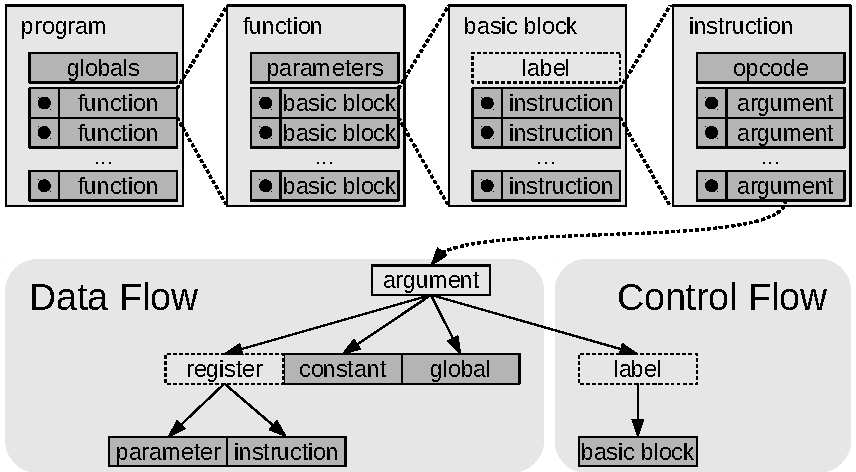
\includegraphics{figures/ssaoverview}
\caption{Structural overview of SSA: Programs are represented as hierarchies of
    lists. The SSA property makes registers implicit, values can be statically
    matched to defining instructions.}
\label{fig:ssaoverview}
\end{figure}

    SSA representations of programs are highly serialised, as shown in
    \autoref{fig:ssaoverview}:
    Programs are lists of functions, functions are lists of basic blocks,
    basic blocks are lists of instructions and instructions are lists of
    arguments.

    The individual instructions operate on an abstract machine, which provides
    an unlimited number of identical registers and a well defined instruction
    set.
    The control flow is expressed as branch instructions, which direct the
    execution conditionally or unconditionally to other basic blocks.
    Basic blocks may have labels or be identified simply by enumerating them.
    Instruction arguments can be registers, constants or globals and branch
    instructions additionally take basic block labels.
    Instructions can write their result into a single output register.
    Branch instructions always terminate a basic block, control flow divergence
    within basic blocks is not possible.

    The static single assignment property stipulates that within a function,
    no register can be written at more than a single static location.
    This makes the data dependencies between the instructions explicit, as it
    implies that registers can be identified directly with the instructions that
    write to them.
    The registers themselves can therefore be considered implicit, with only the
    data flow between instructions required to recover them.

    In the presence of dynamic control flow behaviour in the program, most
    simply in the case of a conditional branch, it is evidently not possible to
    match values to producing instructions statically.
    This is resolved with {\em phi} instructions.
    These instructions select a value from several arguments depending on the
    previously executed basic block, i.e.\ depending on the branch from where
    the execution reached the basic block containing the phi node.

\section{Example of Static Single Assignment Form}

    \autoref{ssaexample} shows many of the key features of static single
    assignment form and how they naturally emerge from simplification steps of
    the source code.
    This is demonstrated on an example function written in C, which appriximates
    the square root function iteratively using the Babylonian method.
    

    Starting from the source code at the top of the figure, the function is
    first simplified by breaking down complex expressions as far as possible.
    This results in a sequentialisation of the expressions into their most basic
    operations, introducing several explicit variables that store the previously
    implicit temporary values.
    The greatly simplifies and normalises the program, with many of the
    remaining simple expressions directly mapping to individual processor
    instructions.

    In a second step, the structured control flow of the program is broken down
    into individual goto statements that coordinate the control between four
    basic blocks.
    While this does not ease the intuitive understanding of the program, it
    unifies the many different control flow structures provided in the source
    language into a single mechanism.
    This makes automatic analysis of the program a less complex task.
    Importantly, no information is lost by discarding the control flow
    structures, as they can be entirely reconstructed with straightforward
    algorithms.

    Lastly, the static single assignment property is introduced.
    Any variable that is assigned in more than one static place in the program
    is instead duplicated into multiple variables.
    These now distinct variables are bound together with $\Phi$ nodes, which
    cannot be expressed in the C syntax.
    Instead, their behaviour is spelled out in the comments in lines 8-9.
    While the impact of the static single assignment property change seems minor
    at first glance, it has many convenient implications.
    As variables are written exactly one, the distinction between local variable
    declarations and definition becomes obsolete.
    This furthermore implies that it is always known statically which expression
    yielded the value of each variable.
    which makes many optimising transformation much less cumbersome to
    implement.
    As a trivial example, this property immediately guarantees that the variable
    $i$ always has the value zero.

    With an understanding of how SSA form emerges during compilation and with,
    it is now the aim to use the serialised nature of it to contruct a
    convenient mathematical model.
    The core observation is that most items in SSA form functions can be easily
    enumerated and identified with by their index.
    This includes the function parameters, expressions and variables.
    After this crucial step, most properties of SSA form functions can be
    described using integers, making for a convenient and easy mathematical
    language.
    
    
    
    

\begin{figure}[p]
\scriptsize
    C source function:
    \begin{lstlisting}[language=C]
double babylonian_method(double square) {
  double root = 1.0;
  for(int i = 0; i < ITER; i++)
    root = 0.5 * (root + square / root);
  return root;
}
    \end{lstlisting}

    Complex expressions are broken down into individual operations:
    \begin{lstlisting}[language=C]
double babylonian_method(double square) {
  double root = 1.0;
  for(int i = 0; i < ITER; i++) {
    double tmp1 = square / root;
    double tmp2 = root + tmp1;
    root = 0.5 * tmp2;
  }
  return root;
}
    \end{lstlisting}

    Structured control flow is expanded into jump statements:
    \begin{lstlisting}[language=C]
double babylonian_method(double square) {
entry:
  double root = 1.0;
  int i = 0;
  goto header;

header:
  bool test = i < ITER;
  if(test) goto body; else goto exit;

body:
  double tmp1 = square / root;
  double tmp2 = root + tmp1;
  root = 0.5 * tmp2;
  i = i+1;
  goto header;

exit:
    return root;
}
    \end{lstlisting}

    The SSA property is introduced:
    \begin{lstlisting}[language=C]
double babylonian_method(double square) {
entry:
  double root = 1.0;
  int i = 0;
  goto header;

header:
  int i_2    = /* reached from 5: i, from 18: i_3 */
  int root_2 = /* reached from 5: root, from 18: root_3 */
  bool test = i_2 < ITER;
  if(test) goto body; else goto exit;

body:
  double tmp1 = square / root_2;
  double tmp2 = root_2 + tmp1;
  double root_3 = 0.5 * tmp2;
  int i_3 = i_2+1;
  goto header;

exit:
    return root_2;
}
    \end{lstlisting}

    \caption{Static Single Assignment emerges from successive simplification
             and normalization of source level features.
             This is demonstrated on an example funtction that approximates the
             square root function with the babylonian method.}
    \label{ssaexample}
\end{figure}

\pagebreak

\section{Deriving a Mathematical Model for SSA}

    In order to develop constraint programming on real world SSA programs with
    mathematical rigour, a sound model is needed first, which will be derived in
    this section.
    It is not the aim here to introduce a formal operational semantics, or more
    generally to derive a model for the execution of SSA programs.
    Instead, the section will investigate the static structure, focusing on
    clear notation of the commonalities of the existing SSA intermediate
    representations.
    The remainder of this section uses the notation in \autoref{not:ssa}.
    Note that no specific representative of the many different SSA languages is
    chosen at this point.

\begin{notation}{Static Single Assignment Function}{ssa}
    For the remainder of this section, some function $\mathcal F$ in SSA form is
    assumed fixed. 
    The following identifiers are then used to describe this function.

    \begin{itemize}
    \item $n_p$ is the number of function arguments $par_1,\dots par_{n_p}$.
    \item $n_i$ is the number of instructions $ins_1,\dots ins_{n_i}$ in the
          function, ordered depth first, starting from the execution entry.
    \item $n_g$ is the number of unique globals $glb_1,\dots glb_{n_g}$ that are
          referenced as an operand of any of the instructions.
    \item $n_c$ is the number of unique constants $cst_1,\dots cst_{n_g}$ that
          are referenced as an operand of any of the instructions.
    \end{itemize}
\end{notation}

    As previously discussed, the static single assignment property makes
    registers implicit.
    All instruction arguments therefore fall into four categories: function
    parameters, constants, globals and other instructions.
    Branching instructions furthermore take basic block labels as brach targets,
    but they can be treated separately.

    For each function, these sets can be statically determined and are finite,
    as implied by \autoref{not:ssa}.
    Therefore, a single integer is enough to encode each instruction argument as
    an index into the union of those four sets.
    Together with the list based representation, this allows for the
    entire argument structure of the instructions in an SSA function to be
    conveniently turned into a labelled multigraph, with edge labels accounting
    for the positional order of the arguments.
    These observations lead to \autoref{def:dfg}.

\begin{definition}{Data Flow Graph}{dfg}
    The {\em data flow graph} of the SSA function $\mathcal F$ is the set
    $DGF_{\mathcal F}\subset \mathbb N^3$ such that
    \begin{align*}
        (a,b,n)\in DFG_{\mathcal F}\iff[1\leq a\leq n_a\land&(arg_a\text{ is the $n$th argument of }ins_b)] \\
                                   \lor[1\leq a-n_a\leq n_i\land&(ins_{a-n_a}\text{ is the $n$th argument of }ins_b)] \\
                                   \lor[1\leq a-n_a-n_i\leq n_g\land&(gbl_{a-n_a-n_i}\text{ is the $n$th argument of }ins_b)] \\
                                   \lor[1\leq a-n_a-n_i-n_g\leq n_c\land&(cst_{a-n_a-n_i-n_g}\text{ is the $n$th argument of }ins_b)].
    \end{align*}
\end{definition}

    Complementing the data flow graph is the control flow graph of the function.
    The control flow graph is usually defined on a basic block granularity, but
    here it will be defined directly on instructions, in order to better
    complement the data flow graph.
    The basic block structure is easily recoverable from this representations.

\begin{definition}{Control Flow Graph}{cfg}
    The control flow graph of the SSA function $\mathcal F$ is the set
    $CGF_{\mathcal F}\subset \mathbb N^3$ such that
    \begin{align*}
        (a,b,n)\in CFG_{\mathcal F}\iff[n=1\land a+1=b\land&(ins_a,ins_b\text{ are in the same basic block})] \\
                                   \lor[(ins_a\text{ terminates a basic block})\land&\\
                                        (ins_b\text{ is the first instruction in the}&\text{ $n$th basic block argument of }ins_a)].
    \end{align*}
\end{definition}

    With the control flow and data flow separated into separate mathematical
    structures, the individual instructions are encoded by their opcodes alone.
    This is demonstrated in \autoref{fig:separation}.
    At the left of the figure is a simple function in an abstract SSA
    representation that calculates an approximation of the square root of
    a number using Newton's method.
    The function has 10 instructions separated into three basic blocks, with the
    majority of the instructions in a loop structure that iteratively improves
    the result.

    The entire information that is encoded in this SSA representation can also
    be recovered from the structures at the right side of the figure:
    per-instruction opcode information, lists of the parameters, constants and
    globals used, the data flow graph as in \autoref{def:dfg} and the control
    flow graph as in \autoref{def:cfg}.

    The only parts of the SSA representation that need to be modeled are the
    per-instruction information, which in this case is nothing more than a list
    of opcodes, and the list of constants, paramters and globals.
    The opcodes are specific to different SSA representations, although a wide
    overlap exists (basic arithmetic, phi nodes).
    For this work, they can simply be modeled as elements of an arbitrary set,
    e.g. $Opcodes_\text{LLVM}$.
    Similarly, $Types_\text{LLVM}$.

\begin{figure}[h]
\begin{minipage}{0.39\textwidth}
\begin{tabular}{|cl|}
\multicolumn{2}{c}{{\bf function} Sqrt($S$)}\\
\hline
{\bf entry} & $\text{goto } loop$\\
\hline
\multirow{8}{*}{\bf loop} & $x \leftarrow \Phi(entry:1,loop:x')$\\
                          & $t_1\leftarrow S/x$\\
                          & $t_2\leftarrow x+t_1$\\
                          & $x'\leftarrow t_2/2$\\
                          & $i\leftarrow \Phi(entry:0,loop:i')$\\
                          & $i'\leftarrow i+1$\\
                          & $c\leftarrow i'+N$\\
                          & $\text{if }c\text{ goto }loop\text{ else }exit$\\
\hline
{\bf exit} & $\text{return }x'$\\
\hline
\end{tabular}
\end{minipage}
\begin{minipage}{0.04\textwidth}
\centering
$\cong$
\end{minipage}
\begin{minipage}{0.22\textwidth}
\begin{tabular}{|l|}
\multicolumn{1}{c}{{\bf function} Sqrt($\square$)}\\
\hline
$\text{goto } \square$\\
$\Phi(\square:\square,\square:\square)$\\
$\square/\square$\\
$\square+\square$\\
$\square/\square$\\
$\Phi(\square:\square,\square:\square)$\\
$\square+\square$\\
$\square+\square$\\
$\text{if }\square\text{ goto }\square\text{ else }\square$\\
$\text{return }\square$\\
\hline
\end{tabular}
\end{minipage}
\begin{minipage}{0.04\textwidth}
\centering
$+$
\end{minipage}
\begin{minipage}{0.27\textwidth}
$par=($`S'$)$\\
$cst=(1,2,0)$\\
$glb=($`N'$)$\\
$CFG=$\\[1pt]{
\tiny\tt\bf
\setlength{\tabcolsep}{1pt}
\renewcommand{\arraystretch}{0.7}
\begin{tabular}{|c|c|c|c|c|c|c|c|c|c|}
\hline
\hphantom{1}&1&&&&&&&&\\[-0.5mm]
\hline
&&1&&&&&&&\\[-0.5mm]
\hline
&&&1&&&&&&\\[-0.5mm]
\hline
&&&&1&&&&&\\[-0.5mm]
\hline
&&&&&1&&&&\\[-0.5mm]
\hline
&&&&&&1&&&\\[-0.5mm]
\hline
&&&&&&&1&&\\[-0.5mm]
\hline
&&&&&&&&1&\\[-0.5mm]
\hline
&1&&&&&&&&2\\[-0.5mm]
\hline
&&&&&&&&&\\
\hline
\end{tabular}}\\[0.75em]
$DFG=$\\[1pt]{
\tiny\tt\bf
\setlength{\tabcolsep}{1pt}
\renewcommand{\arraystretch}{0.7}
\begin{tabular}{|c|c|c|c|c|c|c|c|c|c||c||c|c|c||c|}
\hline
\hphantom{1}&&&\hphantom{1}&&&&&\hphantom{1}&\hphantom{1}&&&&&\\
\hline
2&&&&3&&&&4&&&1&&&\\[-0.5mm]
\hline
&2&&&&&&&&&1&&&&\\[-0.5mm]
\hline
&1&2&&&&&&&&&&&&\\[-0.5mm]
\hline
&&1&&&&&&&&&&2&&\\[-0.5mm]
\hline
2&&&&&&3&&4&&&&&1&\\[-0.5mm]
\hline
&&&&&1&&&&&&2&&&\\[-0.5mm]
\hline
&&&&&&1&&&&&&&&2\\[-0.5mm]
\hline
&&&&&&&1&&&&&&&\\[-0.5mm]
\hline
&&&&1&&&&&&&&&&\\
\hline
\end{tabular}}
\end{minipage}

\caption{Example of DFG and CFG for on a function in abstract SSA representation
         that approximates the square root via Netwon's method.}
\label{fig:separation}
\end{figure}

    With separate mathematical models for all the individual concepts that are
    overlayed in SSA representations, it is now possible to create a complete
    model as shown in \autoref{def:ssamodel}.

\begin{definition}{Mathematical Model of SSA programs}{ssamodel}
    An {\em SSA model} of the SSA function $\mathcal F$ is a tuple
    \begin{align*}
        (DFG_\mathcal{F}, CFG_\mathcal{F},I_\mathcal{F},T_\mathcal{F},C_\mathcal{F},P_\mathcal{F},G_\mathcal{F}),
    \end{align*}
    where $DFG_\mathcal{F}$ and $CFG_\mathcal{F}$ are the data flow and control
    flow graph as in \autoref{def:dfg} and \autoref{def:cfg}.

    $I_\mathcal F\subset\mathbb N\times Opcodes$ is the instruction model, defined by the property
    \begin{align*}
        (k,op)\in I_\mathcal F\iff 1\leq k\leq n_i\land(ins_k\text{ has opcode }op).
    \end{align*}

    $I_\mathcal F\subset\mathbb N\times Types$ is the type model, defined by the property
    \begin{align*}
        (k,ty)\in T_\mathcal F\iff 1\leq k\leq n_i+n_p+n_c+n_g\land(ins_k\text{ has type }ty).
    \end{align*}

    Both $Opcodes$ and $Types$ are implementation specific sets that are not
    further modelled, with elements referred to by name.
    $C_\mathcal F\subset\mathbb N\times\mathbb R$ is the constant model, defined
    by the property
    \begin{align*}
        (k,r)\in C_\mathcal F\iff 1\leq k-n_i-n_p\leq n_c\land(cst_{k-n_i-n_p}\text{ has numeric value equal to }r).
    \end{align*}

    Lastly, $P_\mathcal F\subset\mathbb N$ and $G_\mathcal F\subset\mathbb N$
    are the parameter model and global model that are defined by the properties
    \begin{align*}
        k\in P_\mathcal F\iff& 1\leq k-n_i\leq n_p\text{ and}\\
        k\in G_\mathcal F\iff& 1\leq k-n_i-n_p-n_c\leq n_g.
    \end{align*}

    The set of SSA models is denoted $\mathcal M$.
\end{definition}

    \autoref{fig:derivemaths} shows how this comes together on an example
    program that is represented in a conrete SSA representation.
    At the top of the figure, different textual representations of a simple
    vector dot product are shown.
    The version of the top right is in an SSA intermediate representation: LLVM
    IR as generated by the clang compiler.

\begin{figure}[p]
\centering
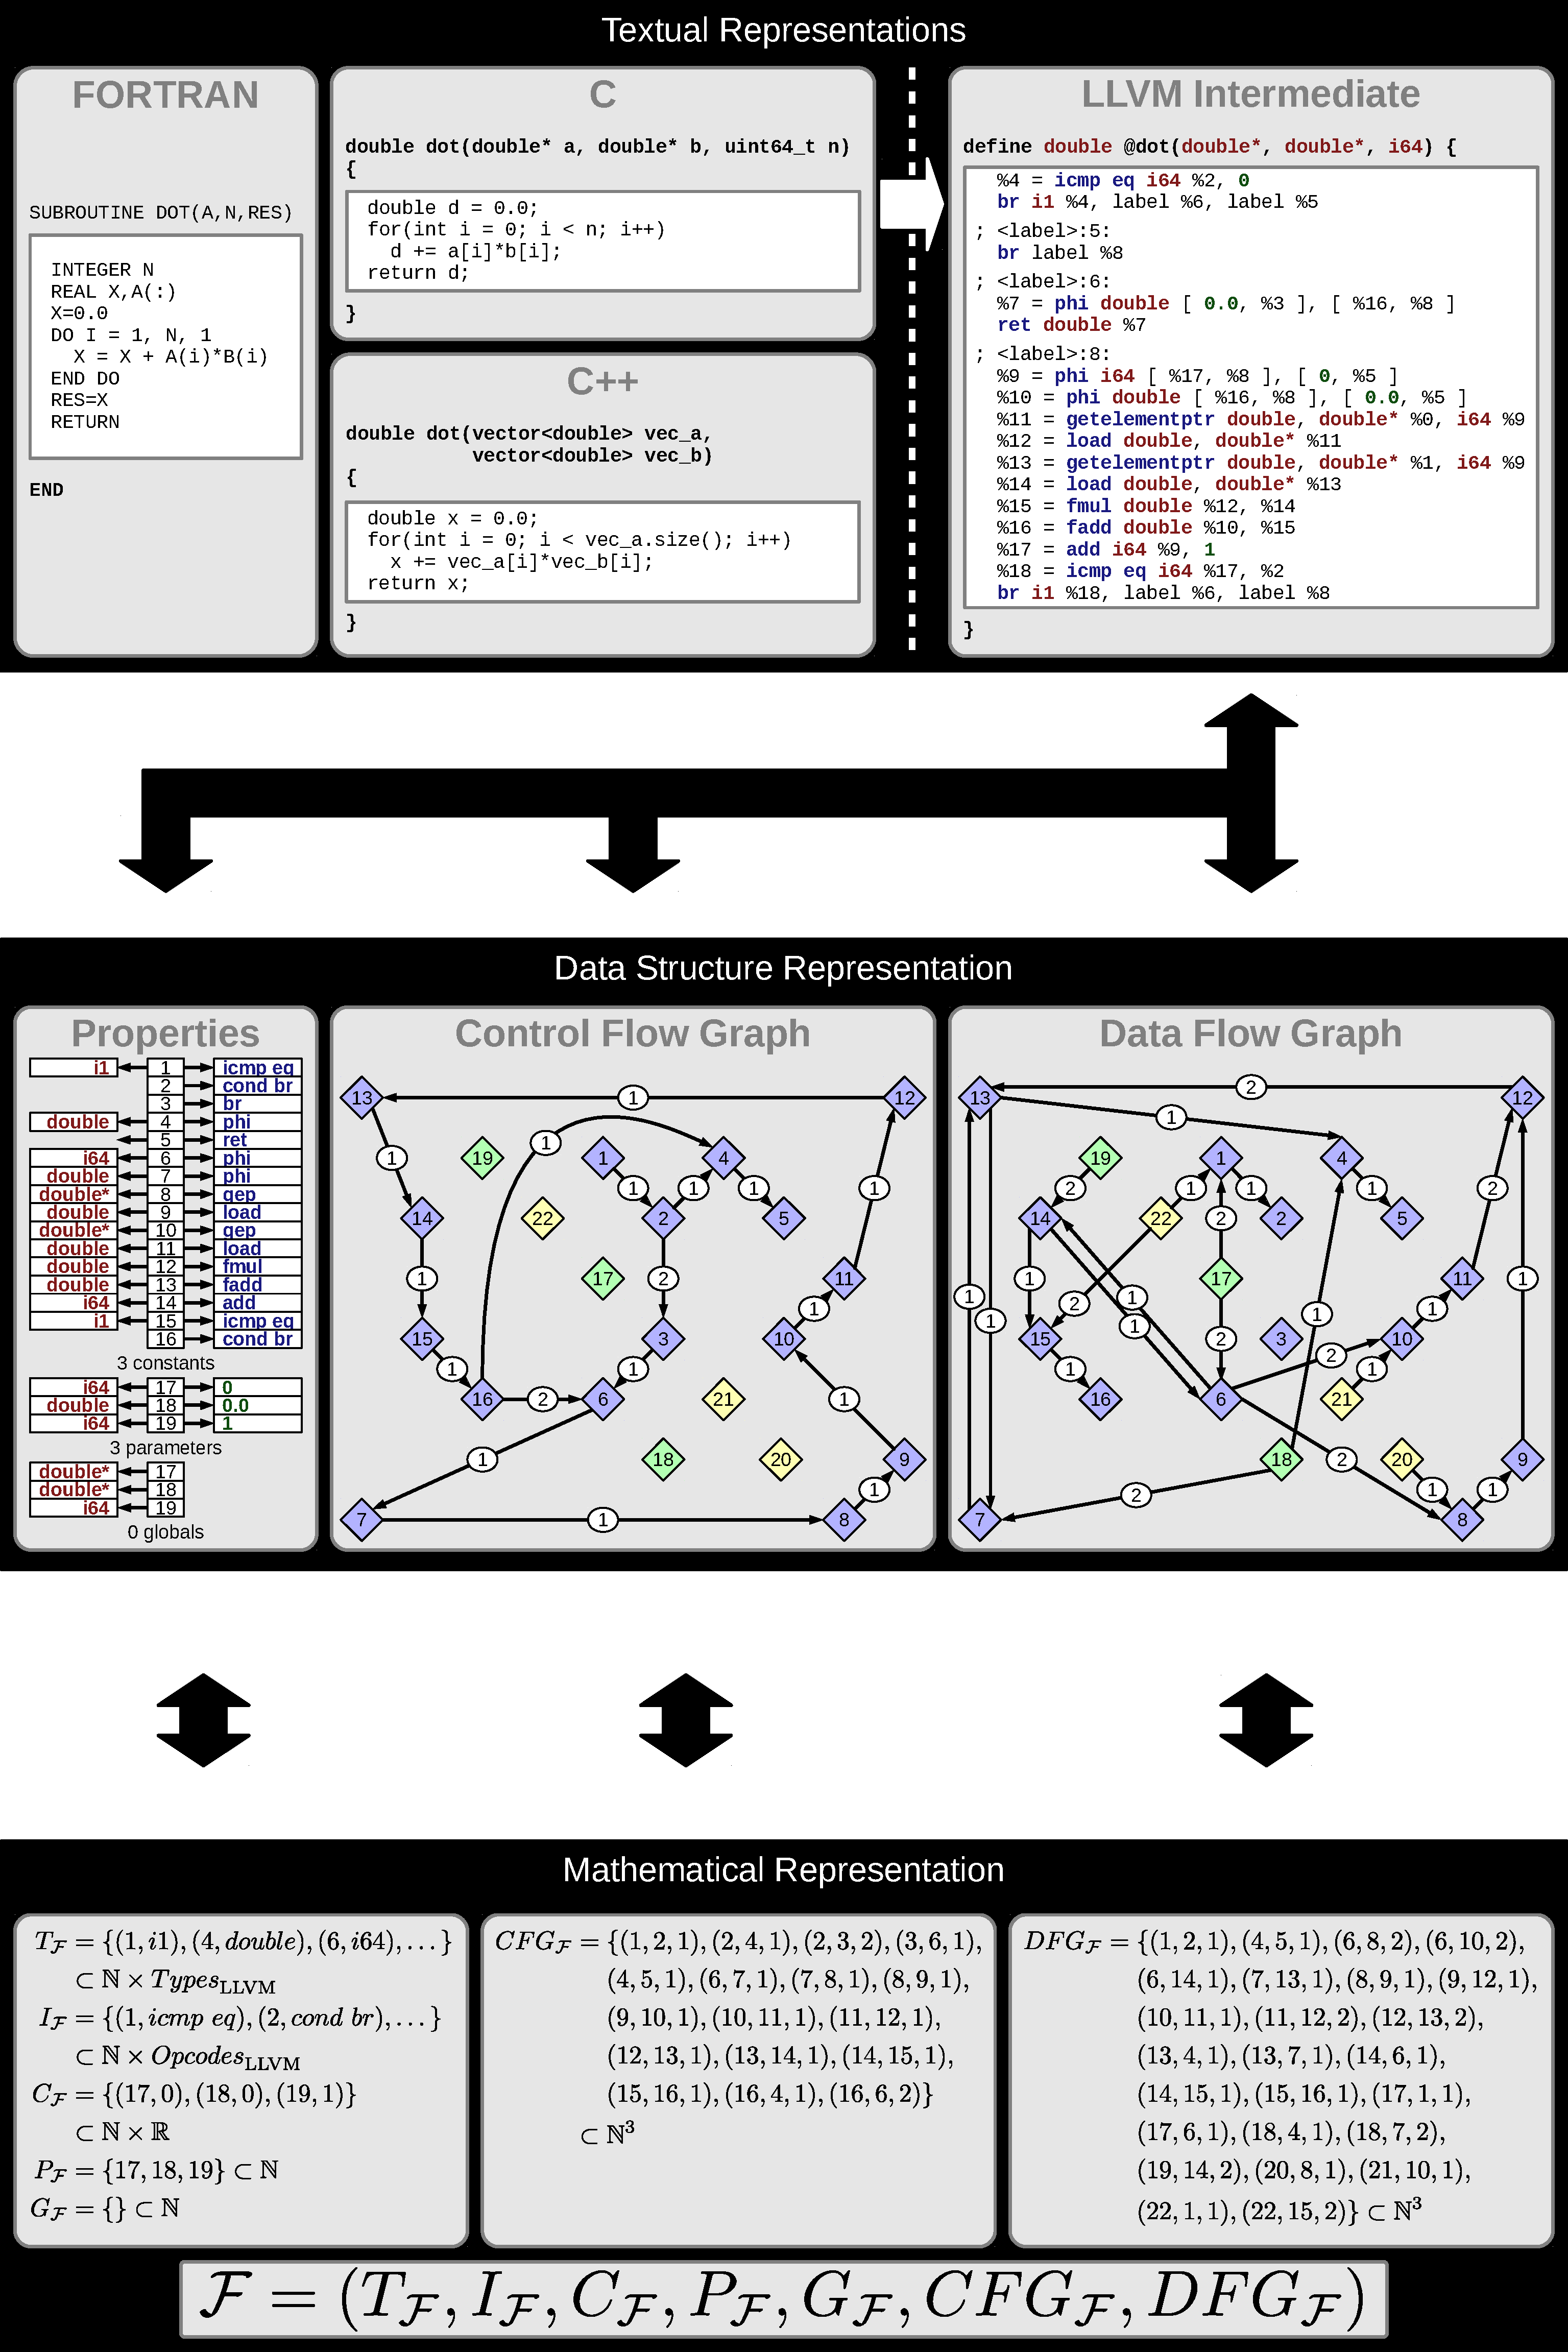
\includegraphics[width=\textwidth,height=1.5\textwidth]{figures/ssamathmodel.pdf}
\vspace{9.31595pt}
\caption{Compiler-generated SSA code is first decomposed into data flow, control
         flow and per-value attributes.
         Mathematical representations of the data are then introduced with
         notation.}
\label{fig:derivemaths}
\end{figure}

    In the middle row of \autoref{fig:derivemaths}, the information contained in
    the SSA representation is split into three components:
    Firstly, the set of per-instruction properties is shown, comprising
    instruction opcodes, types and the values of constants that are used.
    Secondly, the control flow graph is captured.
    Thirdly, the data flow graph of the program is displayed on the right.
    This data structure contains information about how the results of previous
    instructions are used as arguments to successive instructions.
    As we discussed in the previous section, the SSA property ensures that this
    is enough information to make the concrete register usage implicit.

    In the bottom row of \autoref{fig:derivemaths}, the mathematical
    representation of the function is shown, adhering to \autoref{def:ssamodel}.

    To conclude this section, there is some additional notation that will be
    used for convenience later on, listed in \autoref{not:convenience}.

\begin{notation}{Convenient Notation}{convenience}
    For $G\subset\mathbb N^3, k\in\mathbb N$, the following notation applies:
    \begin{align*}
        G^k:=&\{(a,b)\in\mathbb N^2\mid (a,b,k)\in G\}\\
        G^*:=&\{(a,b)\in\mathbb N^2\mid \exists c\in\mathbb N:(a,b,c)\in G\}.
    \end{align*}

    For $G\subset\mathbb N\times\mathbb R, c\in\mathbb R$, the following
    notation applies:
    \begin{align*}
        G^c:=&\{a\in\mathbb N\mid (a,c)\in G\}\\
        G^*:=&\{a\in\mathbb N\mid \exists c\in\mathbb R:(a,c)\in G\}.
    \end{align*}
\end{notation}

\section{Constraint Programming on SSA Programs}

    With a mathematical strucure of SSA models in place, properties of SSA form
    programs can now be formulated as constraint problems.

\begin{definition}{SSA constraint problem}{cprob}

    An SSA constraint problem $C=(V,P)$ is made up of a finite set of variables
    $V$ and a boolean predicate
    $P\colon\mathbb N^V\times\mathcal M\mapsto\{\text{true}, \text{false}\}$.
    The set of {\em constraint solutions} for a given constraint problem and a
    specific SSA model $M\in\mathcal M$ is given as
    \begin{align*}
        S(C,M) = \{s\in\mathbb N^V\mid P(s,M)=\text{true}\}.
    \end{align*}
\end{definition}

    The interesting aspect of this defition is now the structure of $P$.
    This section will concern it self with how meaningful predicates can be
    composed from small building blocks and how the internal structure of the
    predicate can lead to efficient solver approaches.
    In order to evoke an intuition about these challenges, there will first be
    an example.

\subsection{Constraint Program Example}

    Consider the task of detecting in a program all simple loop counters.
    Such loop counters show up in LLVM IR as data flow cycles of a phi node
    and an add instruction.
    We express the constraint problem $C=(V,P)$ with a set of three variables
    $V=\{\text{phi}, \text{update}, \text{step}\}$ and the following predicate:

\begin{figure}
\begin{minipage}{0.4\textwidth}
    \begin{align*}
        V=&\{\text{phi}, \text{update}, \text{step}\}\\
        P(x,\mathcal F)=&(x_\text{phi},x_\text{update})\in DFG_\mathcal{F}^*\land\\
                        &(x_\text{step},x_\text{update})\in DFG_\mathcal{F}^*\land\\
                        &(x_\text{phi}, phi)\in I_\mathcal{F}\land\\
                        &(x_\text{step}, add)\in I_\mathcal{F}\land\\
                        &(x_\text{step},1)\in C_\mathcal{F}\land\\
                        &(x_\text{update},x_\text{phi})\in DFG_\mathcal{F}^*
    \end{align*}
\end{minipage}
\begin{minipage}{0.04\textwidth}
\centering
$\cong$
\end{minipage}
\begin{minipage}{0.22\textwidth}
\begin{tabular}{|l|}
\multicolumn{1}{c}{{\bf function} Sqrt($\square$)}\\
\hline
$\text{goto } \square$\\
$\Phi(\square:\square,\square:\square)$\\
$\square/\square$\\
$\square+\square$\\
$\square/\square$\\
$\Phi(\square:\square,\square:\square)$\\
$\square+\square$\\
$\square+\square$\\
$\text{if }\square\text{ goto }\square\text{ else }\square$\\
$\text{return }\square$\\
\hline
\end{tabular}
\end{minipage}
\begin{minipage}{0.04\textwidth}
\centering
$+$
\end{minipage}
\begin{minipage}{0.27\textwidth}
$par=($`S'$)$\\
$cst=(1,2,0)$\\
$glb=($`N'$)$\\
$CFG=$\\[1pt]{
\tiny\tt\bf
\setlength{\tabcolsep}{1pt}
\renewcommand{\arraystretch}{0.7}
\begin{tabular}{|c|c|c|c|c|c|c|c|c|c|}
\hline
\hphantom{1}&1&&&&&&&&\\[-0.5mm]
\hline
&&1&&&&&&&\\[-0.5mm]
\hline
&&&1&&&&&&\\[-0.5mm]
\hline
&&&&1&&&&&\\[-0.5mm]
\hline
&&&&&1&&&&\\[-0.5mm]
\hline
&&&&&&1&&&\\[-0.5mm]
\hline
&&&&&&&1&&\\[-0.5mm]
\hline
&&&&&&&&1&\\[-0.5mm]
\hline
&1&&&&&&&&2\\[-0.5mm]
\hline
&&&&&&&&&\\
\hline
\end{tabular}}\\[0.75em]
$DFG=$\\[1pt]{
\tiny\tt\bf
\setlength{\tabcolsep}{1pt}
\renewcommand{\arraystretch}{0.7}
\begin{tabular}{|c|c|c|c|c|c|c|c|c|c||c||c|c|c||c|}
\hline
\hphantom{1}&&&\hphantom{1}&&&&&\hphantom{1}&\hphantom{1}&&&&&\\
\hline
2&&&&3&&&&4&&&1&&&\\[-0.5mm]
\hline
&2&&&&&&&&&1&&&&\\[-0.5mm]
\hline
&1&2&&&&&&&&&&&&\\[-0.5mm]
\hline
&&1&&&&&&&&&&2&&\\[-0.5mm]
\hline
2&&&&&&3&&4&&&&&1&\\[-0.5mm]
\hline
&&&&&1&&&&&&2&&&\\[-0.5mm]
\hline
&&&&&&1&&&&&&&&2\\[-0.5mm]
\hline
&&&&&&&1&&&&&&&\\[-0.5mm]
\hline
&&&&1&&&&&&&&&&\\
\hline
\end{tabular}}
\end{minipage}

\begin{align*}
S=\{\{\text{phi}:6,\text{update}:7,\text{step}:12\}\}.
\end{align*}

\caption{Example constraint problem is applied to SSA model from
         \autoref{fig:separation}.
         There is only one simple loop conter in the program, corresponding to
         the loop interator, shown at the bottom.}
\end{figure}

\subsection{Solving of SSA Constraint Problems}

    The aim of a solver for SSA constraint problems is to compute the set of
    solutions $S(C,M)$ for some concrete values of $C$ and $M$.
    This is fundamentally a search problem: the space of $\mathbb N^V$ has to be
    searched for values satisfying $P$.
    The size of $\mathbb N^V$, wich is countable but infinite, requires
    non-trivial computational approaches to this problem, even when the direct
    evaluation of $P$ can be efficiently performed.

    On top of that, an algorithmic solution requires an intelligent way to
    encode the boolean predicate.
    It is intuitive and well established in literature to use backtracking for
    solving constraint problems, so firstly this will be reformulated
    recursively as follows.
    The finite set of $V$ can be enumerated $V=\{v_0,v_1,\dots,v_n\}$.

    Then consider $C_k=(V_k,P_k)$, where $P_k$ is defined as
    \begin{align*}
        P_k(x)=\left\{\begin{array}{l}\text{true} if P(x,y)=true for some y\\
                                      \text{false} otherwise\end{array}\right.
    \end{align*}

    Consider the following purely algebraic reformulation.
    \begin{align*}
        S_k=\{\emptyset\}\\
        S_{k+1}(C,\mathcal F)=&\{s\in\mathbb N^V_k\mid P(s,\mathcal F)=\text{true}\}\\
                             =&\{
    \end{align*}

\subsection{Structure of SSA Constraint Problems}

    Predicates for useful SSA constraint problems are composed by logical
    connectors from a limited set of {\em atomic} predicates, that cannot
    further be decomposed.
    The atomic predicates are defined directly on the mathematical model and
    they often only utilize a very small set of variables, typically one or two.
    Many of then are simple element-of relationships for the different
    components in the SSA model.
    In the previous example, this was true for all the atomic constraints.

    There are some important compiler analysis problems that can not not be
    decomposed with logical connectors into atomic predicates using only one
    or two variables.
    They are mostly concerned with graph properties and we will discuss some of
    them in detail later in this chapter.
    For the purposes of constraint solving, these are more difficult to handle.

    Via the logical connectors $\land$ and $\lor$, the atomic predicates
    interact on their shared variables.
    There will be some additional high level connectors introduced later, which
    appriximate logical operators from first order logic.

\section{Implementation of Constraint Predicates}

    With the solver approach derived, it now needs to be established how real
    constarint problem predicates can be algorithmically implemented in order
    to evaluate the required functions.

\subsection{Important Graph Properties}

    With our established notation, we can now transfer standard compiler
    analysis problems into this more formal language.
    Most of these are based on graph theoretic considerations, so we
    will firstly need to recapitulate some graph theory basics.
    Firstly, there is the notion of {\em cuts} of graphs, that we will introduce
    here in a hybrid version of edge based and vertex based modelling.

    \begin{definition}{Connections and Cuts}{def:cuts}
        Consider an adjacency set $E\subset\mathbb{N}\times\mathbb{N}$ of a
        directed graph and let $a,b\in\mathbb{N}$.
        \newline
        A {\em connection} between $a$ and $b$ in $E$ is a subset
        $A\subset\mathbb{N}$ such that a finite sequence $c_1,\dots,c_n$
        exists with
        \begin{gather*}
            a=c_1\hspace{1cm}c_2,\dots,c_{n-1}\in A\hspace{1cm}b=c_n\\
            (c_k,c_{k+1})\in E\hspace{1em}\text{for all}\hspace{1em}k=1,\dots,n-1.
        \end{gather*}
        A {\em cut} between $a$ and $b$ in $E$ is a subset $B\subset E$
        such that no {\em connection} between $a$ and $b$ in $E\setminus B$
        exists.
        We define the {\em set of cuts} between $a$ and $b$ in $E$ as
        \begin{align*}
            \text{Cuts}_E(a,b):=\{B\subset E\mid B\text{ is {\em cut} between $a$ and $b$ in $E$}\}
        \end{align*}
    \end{definition}

    These notions are quite intuitive, two vertices in a graph have a connection
    if one can reach the other via the available edges and by ``cutting'' these
    edges, they are no longer connected.

    These definitions are very useful in order to identify crucial properties of
    data and control flow graphs.
    Most standard is the the definition of a dominator in the control flow
    graph: An instruction $d$ is said to dominate another instruction $n$ if
    every path from the entry node to $n$ through the control flow graph must
    go through $d$.
    In our model this is of course equivalent to the following:

    \begin{definition}{Dominator}{def:dominator}
        Consider an instruction $n$ in a function $\mathcal F$.
        A {\em dominator} of $n$ in $\mathcal{F}$ is an instruction $d$ such
        that $\{(d,m)\mid(d,m)\in CFG_\mathcal{F}^*\}$ is a {\em cut} between $1$ and $n$ in $CFG_\mathcal{F}^*$.
    \end{definition}

    Another important definition is the concept of control dependence.
    Control dependence models the behaviour of conditional control flow.
    Instructions that are executed only in some control flow paths are control
    dependent on the conditional branches that preceed them.

    \begin{definition}{Control Dependence}{cdg}
        Consider instructions $a,b$.
        We say that an $b$ is control dependent on $a$ if a instructions
        $c,c'$ exist such that $(a,c),(a,c')\in CFG_\mathcal{F}^*$ and
        \begin{align*}
            \{(a,c)\}\in{}&{}\text{Cuts}_E(a,b)\\
            \{(a,c')\}\notin{}&{}\text{Cuts}_E(a,b)\text{.}
        \end{align*}
        We define the {\em control dependence graph} as follows
        \begin{align*}
            CDG_\mathcal{F}:=\{(a,b)\in\mathbb{N}^2\mid b\text{ control dependent on }a\}
        \end{align*}
    \end{definition}

\begin{figure}[p]
    \centering
    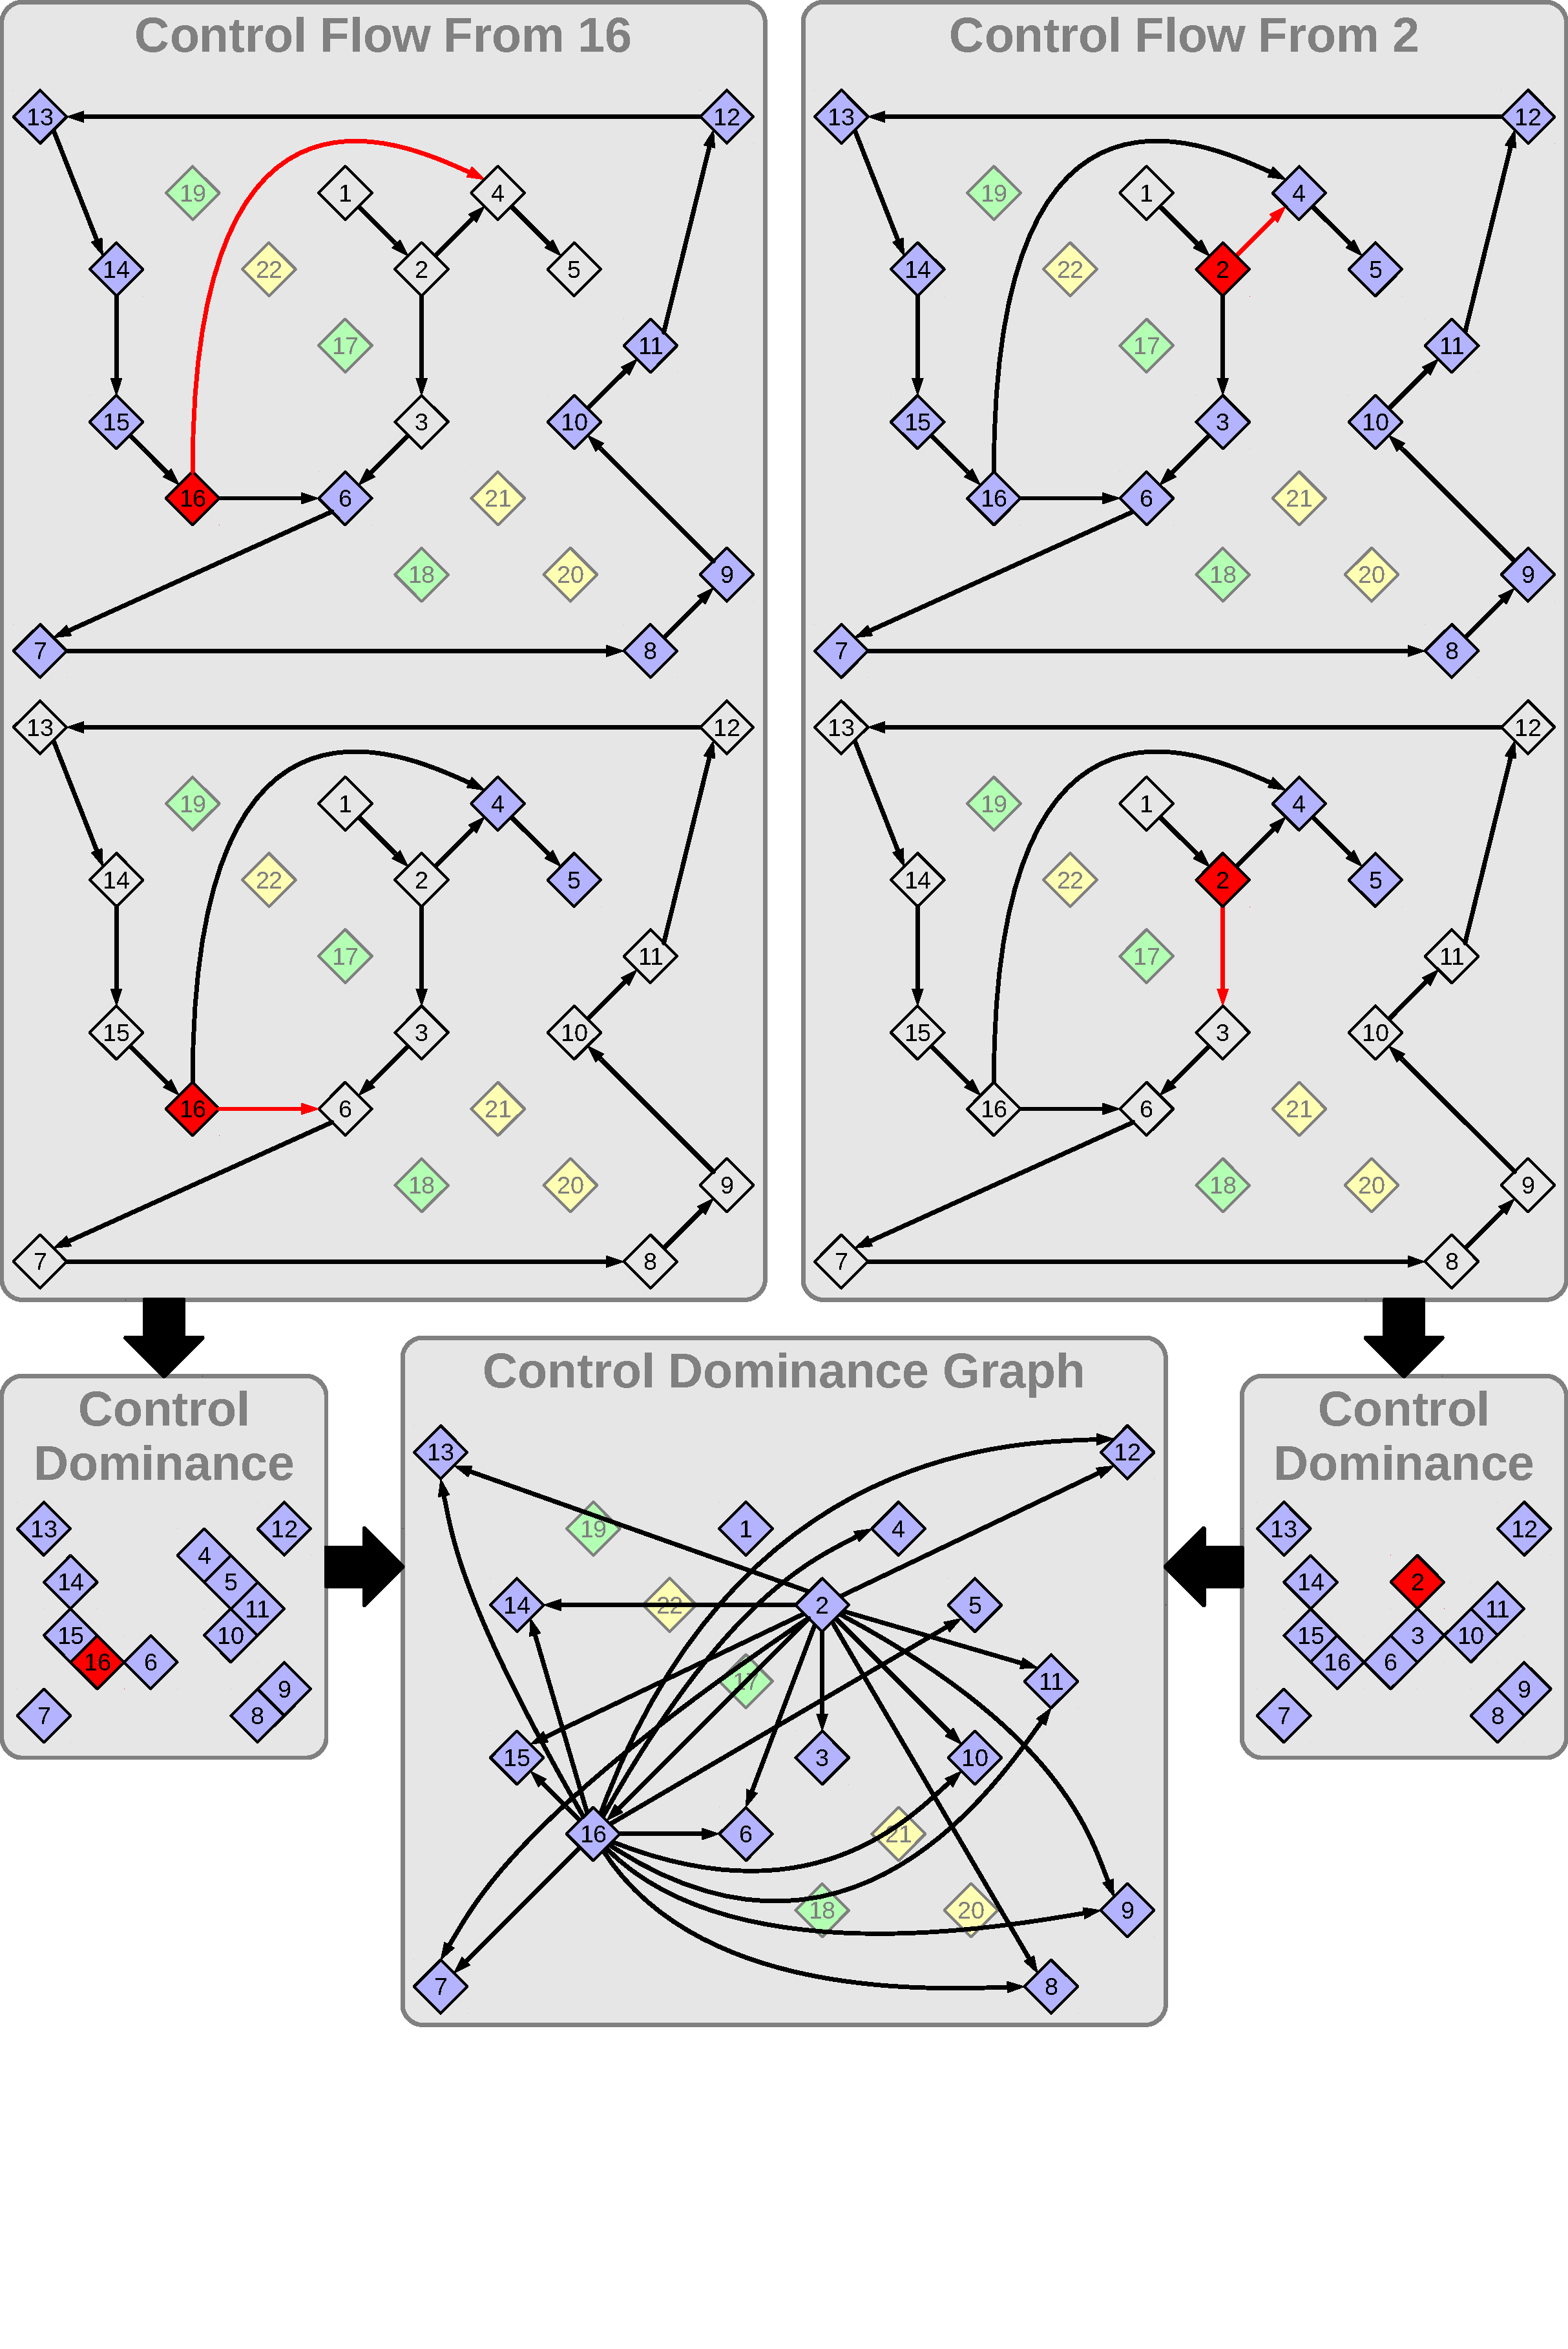
\includegraphics[width=\textwidth,height=1.5\textwidth]{figures/schaubild2.pdf}

    \vspace{27.38136pt}
    \caption{Computation of the control dependence graph.}
    \label{fig:pdg}
\end{figure}


\subsection{Control Dependence Example}

    The control dependence graph is a function of the control flow graph, as is
    directly apparent from \autoref{def:cdg}.
    We can see how an example control dependence graph is computed in
    \autoref{fig:pdg}, from the control flow graph of the \texttt{dot} function
    in \autoref{fig:derivemaths}.
    From the definition it is immediately obvious that we need to only consider
    conditional branches as origins of control dependence.

    We can consider the two conditional branches $2$ and $16$ independently.
    On the right, we consider only $2$.
    We check the defining property: On the top of the figure, all the
    instructions that are not reachable from $2$ without the edge $(2,4)$ are in
    grey.
    Below this, all instructions not reachable from $2$ without $(2,3)$ are
    grey.
    We see that $4,5$ are always reachable and $1$ is never reachable, these are
    therefore not control dependent on $2$.
    All the other instructions are control dependent on $2$.

    Once we have computed this for all conditional branches, we take the union
    on graphs and get the complete control dependence graph of the function.
    Note what this graph represents:
    Once the loop in the function has been unrolled, it contains a conditional
    and a loop.
    Eveything within the body of the conditional is control dependent on $2$.
    Everythig within the loop as well as everything afterwards is control
    dependent on $16$.

\subsection{Phi Dependence Graph}

    Phi nodes are fundamental in single static assignment form and need special
    care.
    The value that a phi node takes depends on from where a phi node was
    reached.
    We need to encapsulate this in a graph.

    \begin{definition}{Phi Dependence Graph}{def:pog}
        Let $p$ a phi node and $c$ a conditional branch instruction.
        We say that the outcome of $p$ depends on $c$ if there is a branch
        instruction $b$ that reaches $p$ such that $b$ is control dependent on
        $c$.

        This defines the {\em phi dependence graph} $\Phi DG_\mathcal{F}$.
    \end{definition}

\subsection{Program Dependence Graph}

    After the control flow, data flow and control dependence graph, we lastly
    introduce the {\em program dependence graph}.
    It is the most exhaustive tool that we have to describe how values depend on
    each other.

    \begin{definition}{Program Dependence Graph}{def:pdg}
        The {\em program dependence graph} is defined as the union of data flow
        and control dependence graphs.
        \begin{align*}
            PDG_\mathcal{F}:=DFG_\mathcal{F}^*\cup CDG_\mathcal{F}^*\cup\Phi DG_\mathcal{F}\text{.}
        \end{align*}
    \end{definition}

    With the program dependence graph, we can now define subsections of the
    program that are self-contained and can be separated into their own
    function.
    This works even if they contain complicated control flow.
    Firstly, we need a definition of an interface.

    \begin{definition}{Interface}{def:interface}
        Let $a\in CFG_\mathcal{F}^*$ and $b_1,\dots,b_n\in DFG_\mathcal{F}^*$.
        Furthermore let $A\subset\mathbb{N}$ a set of instructions.

        We say that $(b_1,\dots,b_n)$ is an interface to $A$ if it is a cut
        between $o$ and $A$ in $PDG_\mathcal{F}$ for any of the following $o$:
        \begin{itemize}
            \item $o$ is a paramter
            \item $o$ is impure
        \end{itemize}
    \end{definition}


\newpage
\subsection{Interface Example}

    We will now consider a non-trivial example.
    Consider this snppet of C code, implementing a function that performs a
    simple square root approximation on each element in an array of double
    precision floating point values.

\begin{figure}[ht]
\begin{lstlisting}[language=C]
void map_sqrt(size_t length, double* array)
{
    for(int i = 0; i < length; i++)
    {
        double root = 1.0;
        for(int i = 0; i < 10; i++)
            root = 0.5*(root+array[i]/root);

        array[i] = root;
    }
}
\end{lstlisting}
\caption{{\bf map$\circ$sqrt}: Apply an appriximate sqare root function to each
         element in a vector.}
\end{figure}

    Coneptually, we should be able to disentangle the square root function from
    the control flow of the outer loop.
    This is possible with the preceeding definition of {\em interfaces}.


\newpage
In single static assignment form, this code looks as follows:

\begin{lstlisting}[language=LLVM]
define void @map_sqrt(i64, double*) {
  %3 = icmp eq i64 %0, 0
  br i1 %3, label %5, label %4

; <label>:4:
  br label %6

; <label>:5:
  ret void

; <label>:6:
  %7 = phi i64 [ %10, %8 ], [ 0, %4 ]
  br label %12

; <label>:8:
  %9 = getelementptr double, double* %1, i64 %7
  store double %19, double* %9
  %10 = add nuw i64 %7, 1
  %11 = icmp eq i64 %10, %0
  br i1 %11, label %5, label %6

; <label>:12:
  %13 = phi i64 [ 0, %6 ], [ %20, %12 ]
  %14 = phi double [ 1.0, %6 ], [ %19, %12 ]
  %15 = getelementptr inbounds double, double* %1, i64 %13
  %16 = load double, double* %15
  %17 = fdiv double %16, %14
  %18 = fadd double %14, %17
  %19 = fmul double %18, 5.0
  %20 = add nuw nsw i64 %13, 1
  %21 = icmp eq i64 %20, 10
  br i1 %21, label %8, label %12
}
\end{lstlisting}

    In this example, the set $\{\%9\}$ is an interface to $\{(\%19,\%store)\}$.

\section{Formulating Constraint Problems}

    With this mathematical background, it is now possible to derive constraint
    programming on top of LLVM code.

    Consider the following definitions of simple binary predicates:

    \begin{align*}
     is\_branch\_inst(\mathcal F, n):= (n,\text{\bf br})\in T_\mathcal{F}\\
     is\_control\_edge(\mathcal F, n, m):= (n,m)\in CFG_\mathcal{F}^*\\
     is\_control\_dom(\mathcal F, n, m):= \\
    \end{align*}

    We can then use these predicates to define more complex constructs, such as
    single entry, single exit (SESE) regions.

    \begin{definition}{}{}{}
        A single entry single exit region is a tuple $a,b,c,d\in\mathcal N$ such
        that the following properties hold:
        \begin{align*}
            is\_control\_edge(\mathcal{F},a,b)\\
            is\_control\_edge(\mathcal{F},c,d)\\
            is\_control\_dom(\mathcal{F},c,d)\\
            is\_control\_postdom(\mathcal{F},d,c)\\
        \end{align*}
    \end{definition}